\documentclass{beamer}
\beamertemplatenavigationsymbolsempty
\usepackage[french]{babel}
\usepackage{fontspec}
\usepackage{amsmath, amsthm, amsfonts}
\usepackage[separate-uncertainty]{siunitx}
\usepackage{xcolor}
\usepackage{tikz}
\usepackage{tikz-cd}
\usepackage[object=vectorian]{pgfornament}
\usepackage{circuitikz}
\usepackage{hyperref}
\usepackage{caption}
\usepackage{booktabs}
\usepackage{mathtools}
\usepackage{longtable}
\usepackage[version=3]{mhchem}
\usepackage{marginnote}
\usepackage[framemethod=tikz]{mdframed}


% Paul Tol's qualitative palette
% ``bright''.https://personal.sron.nl/~pault/#sec:qualitative
\definecolor{tblue}{HTML}{4477AA}
\definecolor{tcyan}{HTML}{66CCEE}
\definecolor{tgreen}{HTML}{228833}
\definecolor{tyellow}{HTML}{CCBB44}
\definecolor{tred}{HTML}{EE6677}
\definecolor{tpurple}{HTML}{AA3377}
\definecolor{tgrey}{HTML}{BBBBBB}


% Justification for marginnotes.
\renewcommand*{\raggedleftmarginnote}{}
\renewcommand*{\raggedrightmarginnote}{}


% Styles for mdframed environments.
\newmdenv[backgroundcolor=tgreen!10,linecolor=tgreen!30]{reponsebox}
\newmdenv[backgroundcolor=tyellow!10,linecolor=tyellow!30]{diapobox}
\newmdenv[backgroundcolor=tred!10,linecolor=tred!30]{fondamentalbox}

% Default arrow for tikz and style for positive and negative objects.
\tikzset{>=latex,
    negative/.style={draw=teal!70!black, fill=teal!10, thick},
    positive/.style={draw=red, fill=red!10, thick}}
\usetikzlibrary{matrix,calc,decorations.pathreplacing,decorations.pathmorphing,decorations.markings}

% French locale for numbers and negative exponent for units.
\sisetup{locale=FR, per-mode=symbol}

\newcommand{\abs}[1]{\left| #1 \right|}
\newcommand{\rhat}{\vec{\hat{r}}}
\newcommand{\xhat}{\vec{\imath}}
\newcommand{\yhat}{\vec{\jmath}}
\newcommand{\zhat}{\vec{k}}
\newcommand{\real}{\mathbb{R}}
\newcommand{\der}[2]{\frac{\mathrm{d}#1}{\mathrm{d}#2}}
\newcommand{\pder}[2]{\frac{\partial\ #1}{\partial\ #2}}
\newcommand{\dif}{\mathrm{d}}
\newcommand{\ddif}{\,\mathrm{d}}
\newcommand{\grad}{\vec{\nabla}}
\newcommand{\exemple}[1]{\begin{fullwidth}#1\end{fullwidth}}
\newcommand{\norm}[1]{\lVert\ #1\ \rVert}
\newcommand{\vu}{\vec{u}}
\newcommand{\vv}{\vec{v}}
\newcommand{\vr}{\vec{r}}
\newcommand{\va}{\vec{a}}
\newcommand{\vF}{\vec{F}}
\newcommand{\vE}{\vec{E}}
\newcommand{\vB}{\vec{B}}
\newcommand{\vecxyz}[3]{#1 \xhat\ + #2 \yhat\ + #3 \zhat}
\newcommand{\vecxy}[2]{#1 \xhat\ + #2 \yhat}
\newcommand{\coulombcst}{k}
\newcommand{\emf}{\ensuremath{\mathcal{E}}}
\newcommand{\eval}{\SI{1.602e-19}{C}}
\newcommand{\kval}{\SI{8.99e9}{Nm^2 \per C^2}}

% Nice separator line
\newcommand{\sectionline}{
    \noindent
    \begin{center}
        \resizebox{0.5\linewidth}{1ex}
    {{%
    {\begin{tikzpicture}
    \node  (C) at (0,0) {};
    \node (D) at (9,0) {};
    \path (C) to [ornament=85] (D);
    \end{tikzpicture}}}}
    \end{center}
}

\theoremstyle{definition}
\newtheorem*{defn}{Definition}


\usepackage[version=3]{mhchem}

\setbeamercolor{title}{fg=tblue}
\setbeamercolor{frametitle}{fg=tblue}
\setbeamercolor{structure}{fg=tblue}

% Make footnotesize smaller
\makeatletter
\renewcommand\footnotesize{%
   \@setfontsize\footnotesize\@viipt{11}%
   \abovedisplayskip 8\p@ \@plus2\p@ \@minus4\p@
   \abovedisplayshortskip \z@ \@plus\p@
   \belowdisplayshortskip 4\p@ \@plus2\p@ \@minus2\p@
   \def\@listi{\leftmargin\leftmargini
               \topsep 4\p@ \@plus2\p@ \@minus2\p@
               \parsep 2\p@ \@plus\p@ \@minus\p@
               \itemsep \parsep}%
   \belowdisplayskip \abovedisplayskip
}
\makeatother

\title{Électricité et magnétisme}
\subtitle{Chapitre 9 - Force magnétique}
\date{23 novembre 2021}
\author{Loïc Séguin-Charbonneau}
\institute{Cégep Édouard-Montpetit}

\begin{document}

\maketitle

\begin{frame}{Proton et fil}
  Un proton a une vitesse parallèle à un long fil parcouru d'un courant $i$. La
  vitesse du proton est dans la même direction que le courant.
    \begin{center}
      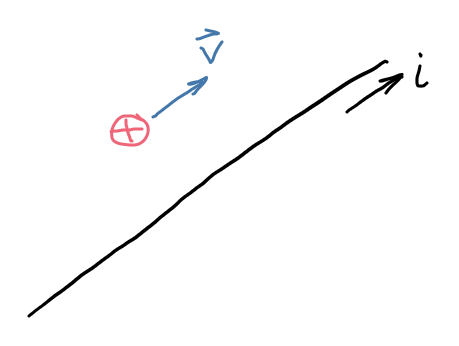
\includegraphics[scale=0.3]{figures/proton_fil.png}
    \end{center}
  Le proton 
  \begin{enumerate}[A.]
    \item<alert@2> se rapprochera du fil
    \item s'éloignera du fil
    \item continuera son chemin en ligne droite
  \end{enumerate}
\end{frame}


\begin{frame}{Électron et fil}
  Un électron a une vitesse perpendiculaire à un long fil parcouru d'un courant
  $i$.
  \begin{center}
    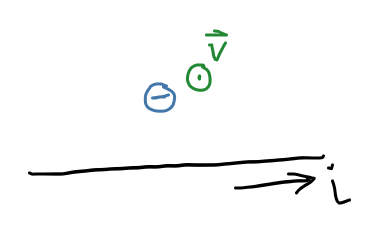
\includegraphics[scale=0.3]{figures/electron_fil.png}
  \end{center}
  La force sur l'électron est 
  \begin{enumerate}[A.]
    \item vers le fil
    \item parallèle au fil
    \item<alert@2> nulle
    \item pointe en s'éloignant du fil
  \end{enumerate}
\end{frame}


\begin{frame}[t]{Exercice}
On envoie des particules avec une vitesse horizontale de \SI{3.52e5}{m/s} dans
une région où existe un champ magnétique uniforme de \SI{1}{G} vers le bas. On
observe qu'à leur arrivée dans le champ magnétique, les particules tournent
dans le sens horaire lorsqu'on les regarde du dessus. Le rayon de leur
trajectoire est de \SI{2}{cm}.

\begin{enumerate}
  \item Déterminer le signe de la charge de ces particules.
  \item Déterminer le rapport $q/m$ pour ces particules.
  \item Déterminer la fréquence de leur mouvement.
\end{enumerate}
\end{frame}


\begin{frame}[t]{Exercice}

Des particules $\alpha$ sont envoyées dans une région où se trouvent un champ
électrique uniforme de \SI{236}{V/m} et un champ magnétique uniforme
perpendiculaire de \SI{155}{mT}. Quelle est l'énergie cinétique des particules
$\alpha$ qui continuent leur trajectoire en ligne droite?

\end{frame}


%\begin{frame}[t]{Exercice}

%On considère un spectromètre de masse avec un champ magnétique de \SI{10}{G}.
%On envoie des ions +1 de nickel 58 (\SI{57.935}{u}) et de nickel 60
%(\SI{59.931}{u}).  Un sélecteur de vitesse s'assure que la vitesse de tous les
%ions est de \SI{1e5}{m/s}. Quelle est la distance entre les points où arrivent
%les deux isotopes de nickel?

%\end{frame}


\begin{frame}{Fil dans un champ magnétique}

  Une section de fil de \SI{8}{\centi\meter} parcouru d'un courant de
  \SI{10}{\ampere} se trouve dans un champ magnétique uniforme de
  \SI{5}{\tesla}. Quelle est la force sur le fil?

  \begin{center}
    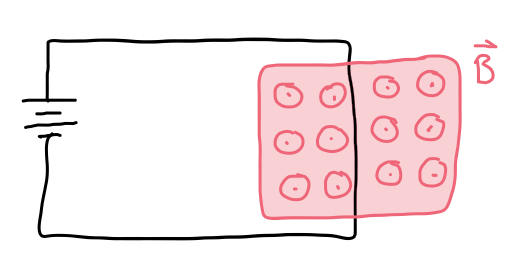
\includegraphics[width=5cm]{figures/fil_dans_mag.png}
  \end{center}
\end{frame}


\begin{frame}{Force entre deux fils}
  Une section de fil de \SI{8}{\centi\meter} parcouru d'un courant de
  \SI{10}{\ampere} se trouve à proximité d'une section de fil parallèle de même
  longueur parcouru d'un courant de \SI{5}{\ampere}. Les deux fils sont séparés
  d'une distance de \SI{2}{\centi\meter}.
  \begin{center}
    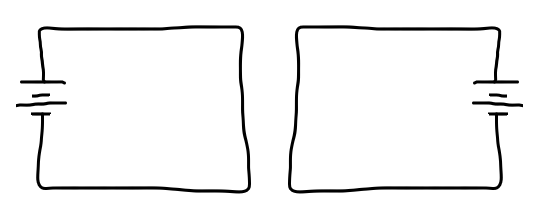
\includegraphics[width=5cm]{figures/deux_fils.png}
  \end{center}
  \begin{enumerate}
    \item Quelle est la force sur le fil de gauche?
    \item Quelle est la force sur le fil de droite?
  \end{enumerate}
\end{frame}


\begin{frame}{Boucle dans un champ magnétique}
  \begin{center}
    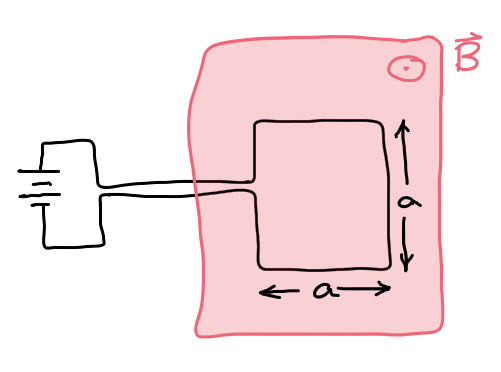
\includegraphics[width=5cm]{figures/boucle_dans_mag.png}
  \end{center}

  \only<1-2>{
    Déterminer la force magnétique sur la boucle.

    \begin{enumerate}[A.]
      \item $iaB$
      \item $4iaB$
      \item $ia^2B$
      \item<alert@2> $0$
    \end{enumerate}
  }

  \only<3-4>{
    Est-ce que la boucle tournera?

    \begin{enumerate}[A.]
      \item Oui, la partie du haut s'approchera de nous
      \item Oui, la partie du haut s'éloignera de nous
      \item Oui, la partie de droite s'approchera de nous
      \item<alert@4> Non
    \end{enumerate}
  }
\end{frame}


\begin{frame}{Boucle dans un champ magnétique}
  \begin{center}
    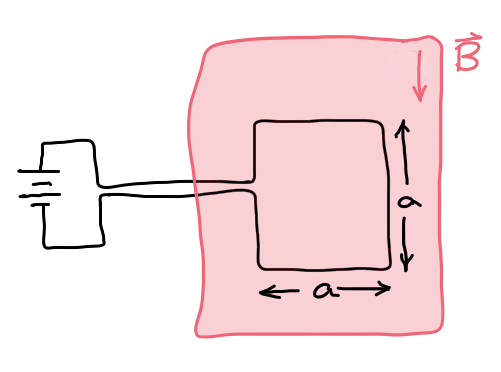
\includegraphics[width=5cm]{figures/boucle_dans_mag_2.png}
  \end{center}

  \only<1-2>{
    Déterminer la force magnétique sur la boucle.

    \begin{enumerate}[A.]
      \item $iaB$
      \item $4iaB$
      \item $ia^2B$
      \item<alert@2> $0$
    \end{enumerate}
  }

  \only<3-4>{
    Est-ce que la boucle tournera?

    \begin{enumerate}[A.]
      \item Oui, la partie du haut s'approchera de nous
      \item<alert@4> Oui, la partie du haut s'éloignera de nous
      \item Oui, la partie de droite s'approchera de nous
      \item Non
    \end{enumerate}
  }
\end{frame}

\end{document}

